\chapter{Results and discussion}
\label{cha:result}

\section{Energy-saving path finding}
\label{sec:result_project1}
The test environment is a 100x100 2D space given in figure \ref{fig:envs}, 
Without any floating objects in the space, each point is dedicated a value indicating the height of the obstacle of the point (0 means plain ground with no obstacles). 
For simplicity, only square obstacles are considered as shown in the figures.



\begin{figure}[!htb]
    \centering
    \begin{subfigure}[b]{.475\textwidth}
        \centering
        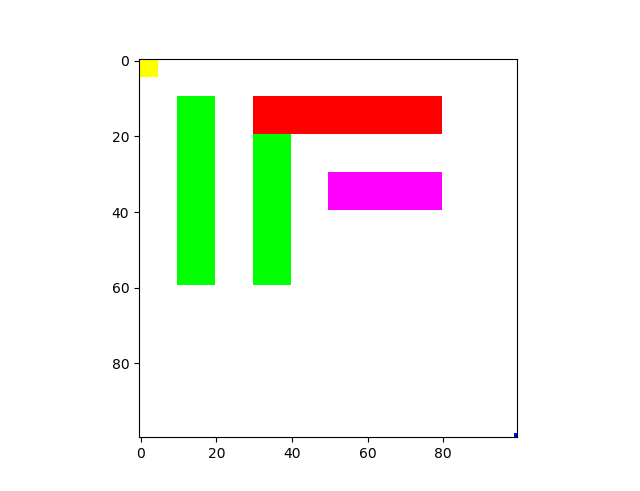
\includegraphics[width=\textwidth]{Figs/env1.png}
        \caption{The robot should pass the green obstacle}
        \label{fig:env1}
    \end{subfigure}%
    \hfill
    \begin{subfigure}[b]{.475\textwidth}
        \centering
        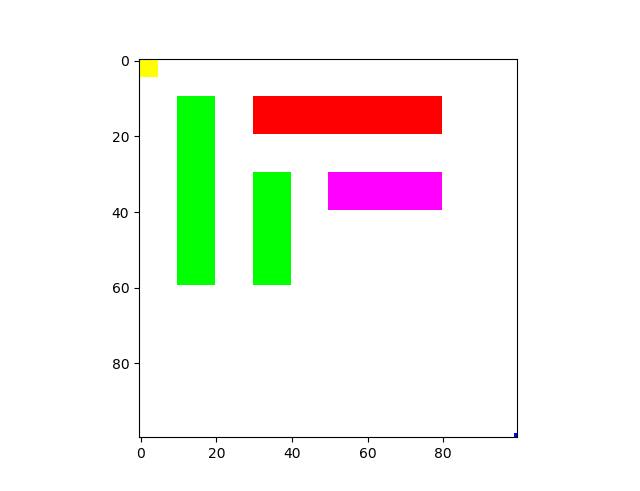
\includegraphics[width=\textwidth]{Figs/env2.png}
        \caption{The robot should avoid the green obstacle}
        \label{fig:env2}
    \end{subfigure}
    \vskip\baselineskip
    \begin{subfigure}[b]{.475\textwidth}
        \centering
        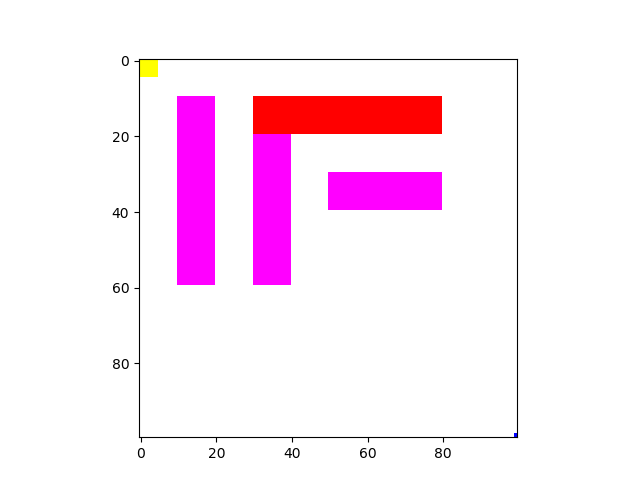
\includegraphics[width=\textwidth]{Figs/env3.png}
        \caption{The robot should choose to detour}
        \label{fig:env3}
    \end{subfigure}%
    \hfill
    \begin{subfigure}[b]{.475\textwidth}
        \centering
        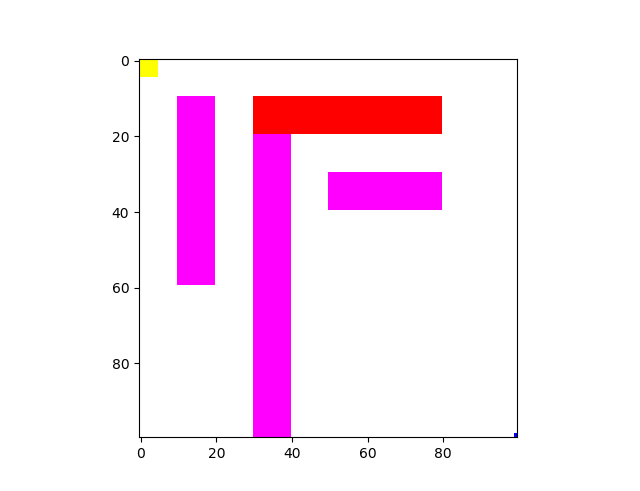
\includegraphics[width=\textwidth]{Figs/env4.png}
        \caption{The robot should pass the purple obstacle}
        \label{fig:env4}
    \end{subfigure}
    \caption{Test environments}
    \label{fig:envs}
\end{figure}

Green color represents obstacles that are easy to pass. 
So the robot should choose to pass the green obstacles if the detour is not too long. (figure \ref{fig:env1} and \ref{fig:env2})

Purple color represents obstacles that are difficult to pass and red color represents obstacles that are impossible to pass.
So the robot should choose to detour around purple obstacles unless the detour is extremely long. (figure \ref{fig:env3} and \ref{fig:env4})
The parameters should be chosen to make the robot make same decisions as indicated in the captions.

\section{Multi-arm robot}
\label{sec:result_project2}